\chapter{Introduction}
\label{introduction}

%\dropcap{E}ver since its introduction in 1983, the Internet has grown to a global communication network used by individuals to interact with others.
%Nowadays, numerous companies operate large-scale digital platforms to facilitate on-line interactions between potentially billions of users.
%eBay was one of the first platforms that enabled the trustworthy trade of goods between merchants and buyers over the Internet, and is used by millions on a daily basis.
%More recently, companies acting in the sharing economy, like Uber and AirBnb, shaped the notion of digital interactions between individuals over the Internet.
%These companies facilitate peer-to-peer resource sharing where strangers can share personal resources, like their house or car, in a trustworthy manner.

%Most of the on-line applications we use on a daily basis are \emph{centralized}, e.g., managed by a single authority that maintains the required network infrastructure. % facilitated by centralized architectures, often deployed and maintained by a single company.
%In particular, when considering a centralized Internet application, there is a single or limited group of servers, responsible for processing all requests submitted by the platform participants, e.g., uploading a video on YouTube or posting a tweet on Twitter.
%Hosting the network infrastructure to facilitate interactions on a global scale requires major investments and platform costs, as exemplified by major companies like Facebook and Google.
%On one hand, centralized infrastructures are relatively easy to setup and their performance can be increased by deploying more servers.
%On the other hand, even a single software bug or hardware failure could lead to a prolonged unavailability of the entire application.
%For example, Facebook experienced a day of downtime in March 2019 due to a server misconfiguration.

%In comparison, \emph{decentralized} applications aim to avoid reliance on a single authority.
%A decentralized application consists of a network where computers directly communicate and collaborate with each other instead.
%One of the most popular decentralized applications is the BitTorrent file transfer protocol, used to share and download torrent files.
%In BitTorrent, users directly exchange parts a (potentially large) file with each other over the network, without any requirement for servers that are under the control of a single authority.
%Although the global unavailability of a decentralized application is a rare phenomena, they often are more vulnerable to attacks targeted at the network layer, such as the Sybil Attack and the Eclipse Attack.

\dropcap{M}arketplaces facilitate the exchange of services, goods and information between individuals and businesses.
They play an essential role in our economy, enabling the exchange of value on both a local and a global scale.
A large part of all conducted trades proceeds on electronic marketplaces that leverage Internet technology to electronically buy or sell products and digital services.
On electronic marketplaces, users routinely trade with other users with whom they never interacted before, unlike in many physical marketplaces.
%The Internet provides the infrastructure to globally exchange information and to deploy large-scale electronic marketplaces, e.g., Amazon and eBay.
Amazon and eBay are well-known examples of large-scale electronic marketplaces that facilitate the exchange of goods between buyers and sellers.
During the last decades, companies acting in the \emph{sharing economy}, such as Uber and AirBnb, have further expanded the impact of e-commerce by offering global marketplaces for the sharing of personal resources such as cars and houses with strangers.
%During the last decade, this effect has been amplified by companies acting in the \emph{sharing economy}, like Uber and AirBnb.
%The notion of sharing personal resources with strangers (e.g., cars and houses) has long been perceived as unreliable.

%In general, the role of marketplaces, electronic and otherwise, is three-fold~\cite{bakos1998emerging}.  % https://dl.acm.org/doi/pdf/10.1145/280324.280330
%First, they have to match buyers and sellers, either through an automated matchmaking process or by offering the required functionality for users to browse through the services or goods offered on the market.
%Second, the market has to facilitate transactions, including the delivery of goods from a seller to a buyer and associated payment flows.
%Third, the market has to provide institutional infrastructure for fraud management, dispute resolution and regulatory compliance.

The standard approach to devise electronic marketplaces is by deploying centralized infrastructure, entirely operated and managed by an authoritative market operator.
This market operator provides the required primitives for bringing buyers and sellers together, for the management of market information (e.g., product listings), and for transaction processing (e.g., by providing payment services).
Also, the market operator often acts as a trusted intermediary between buyers and sellers, leveraging its intermediate position to address potential conflicts arising between traders.
For example, the ride-hailing company Uber ensures that its drivers are sufficiently qualified to offer their services to passengers, mediates in case of a dispute, and processes all payments made by passengers.
Market intermediaries usually charge users for the provided services through transaction fees.

Advancements in information technology, in particular blockchain technology, have challenged the need for both authoritative market operators and trusted intermediaries.
The Bitcoin currency, powered by a tamper-proof distributed ledger, has demonstrated that it is possible to build a cash system, not under the ownership of a financial institution~\cite{nakamoto2008bitcoin}.
Similarly, Ethereum enables developers to write legally-binding contractual logic without notaries~\cite{wood2014ethereum}.
As we will elaborate, the notion of \emph{disintermediation}, removing trusted intermediaries, is closely related to the process of \emph{decentralization} where authority residing in a single entity is re-distributed over multiple entities.
There is an increasing amount of research effort to disintermediate different aspects of electronic marketplaces and to replace centralized components with decentralized solutions, such as distributed ledgers.

% TODO logische volgorde: information management -> matchmaking -> settlement -> fraud mangement -> identity management

This thesis introduces novel mechanisms for decentralization and disintermediation in blockchain-based marketplaces.
%A key characteristic of such blockchain-based marketplaces is that economic activity emerges from the direct interactions between buyers and sellers with minimal involvement of trusted intermediaries.
We design, implement, evaluate and deploy five decentralized mechanisms that improve different aspects of existing blockchain-based marketplaces.
These aspects are information management, matchmaking, settlement, fraud management, and identity management.
Each introduced mechanism focusses on one or more of these aspects.
In the remainder of this introduction, we define the concepts of decentralization and disintermediation in the context of this thesis, and elaborate on the five aspects of blockchain-based marketplaces.
%While the discussed mechanisms in this thesis focus on different aspects of marketplaces, their common goal is to identify the role of trusted intermediaries and assess if theyr . 
%The remainder of this introduction is structured as follows:, we first outline the impact of the Internet as infrastructure to conduct trade.
%Next, we show how blockchain technology makes it possible to devise marketplaces without middleman.
%Then, we discuss the critical components of blockchain-based marketplaces and present existing approaches to realise each component.
%Finally, we state the main research question that this thesis answers.

\section{Decentralization in Blockchain-based Markets}
\label{sec:decentralization}
This thesis discusses five decentralized solutions for blockchain-based marketplaces.
Therefore, it is important to understand what decentralization means in the context of this thesis, and how blockchain-based marketplaces achieve decentralization.
%Specifically, we define the term \emph{decentralization} in the context of this work, and show how this concept is applied by blockchain-based marketplaces.

\subsection{What is Decentralization?}
The anonymous communication protocol Tor~\cite{syverson2004tor} and the digital currency Bitcoin~\cite{nakamoto2008bitcoin} are prominent examples of decentralized Internet solutions that have seen successful adoption.
At the same time, there is no established, standard definition of decentralization within the context of Internet-deployed systems.
Decentralization is defined by Merriam-Webster as \enquote{the dispersion or distribution of functions and powers}.
It describes the process by which decision making is delegated away from a central, authoritative entity, for example, delegating decision making from a government to provinces or municipalities within a country.
Decentralization is widely used as a term within different branches of science, including economics, social sciences and computer science.

In computer science, the term decentralization is increasingly being used to indicate systems where decisions are not taken by a single entity and where the authority is spread over the participants in the network.
Decentralization is usually accredited as a desirable property of a computer system, reducing privacy threats and raising the bar to manipulate and take down the entire system by adversarial actors~\cite{troncoso2017systematizing}.
To date, however, the vast majority of popular Internet applications are centralized systems, e.g., YouTube, Netflix and Facebook.
During the last decade, these so-called \enquote{Big Tech} companies have accumulated an unprecedented amount of power and market share.
A key advantage of centralized systems is that they are relatively easy to setup and maintain, in stark contrast to decentralized networks.
%The original vision of the Internet is an example of a decentralized systems, consisting of many autonomous, interlinked nodes.

\subsection{Blockchain Technology}
Blockchain technology has profoundly shaped the notion of decentralization within the domain of distributed systems~\cite{aste2017blockchain}.
In 2008, Satoshi Nakamoto\footnote{A pseudonym. The real identity behind the pseudonym is unknown.} introduced the Bitcoin cryptocurrency, a peer-to-peer cash system without banks~\cite{nakamoto2008bitcoin}.
Bitcoin challenged what has long been thought to be an impossible problem: reaching distributed consensus in open, large-scale networks without trusted intermediaries.
At the core of Bitcoin is a \emph{blockchain}, a distributed ledger that is fully secured and maintained by participating users.
The blockchain is a chain consisting of blocks, and each block contains one or more transactions.
Each block, except for the first one, is equipped with a hash pointer that points to the previous block.
This pointer makes the blockchain structure tamper-evident since the modification of historical transactions can efficiently be detected.
%This profoundly shaped the way in which distributed systems are designed.
%Bitcoin is the first electronic cash system with significant adoption, compared to similar proposals, and has gained much interest from both academia and industry.
%Bitcoin is the first system to enable the controlled minting of digital cash without a bank.
%Ten years later, blockchain technology is being researched within a large number of domains, including finance, health care, identity and real estate.
%In particular, there has been much interest from the open-source developer community to build and deploy decentralized applications powered by blockchain technology.
%At the time of writing, there are \todo{X} decentralized applications running only on the Ethereum blockchain.

The Bitcoin network maintains a blockchain that records all transactions ever made.
In Bitcoin, users submit signed transactions and pay fees to get their transactions embedded in the blockchain.
A particular group of users, also called \emph{miners}, reach \emph{consensus} on which block and transactions enter the blockchain.
This works as follows: miners periodically propose a new block with transactions to be appended to the current blockchain.
Each miner competes with other miners by solving a computational puzzle derived from the proposed block, a process also called \emph{block mining}.
This puzzle involves finding a hash that satisfied a certain condition, for example, it starts with a number of leading zeros.
The first miner to present a block with a correct hash to the network can append its proposed block and gets rewarded with a fixed number of Bitcoin (this number decreases over time).
Furthermore, the winning miner can claim all transaction fees of the transactions within the block.
The parameters in this consensus algorithm, also called \emph{Proof-of-Work} (PoW) or \emph{Nakamoto consensus}, are fixed such that a new block is created roughly every ten minutes.

Despite significant hype surrounding the Bitcoin ecosystem and its tremendous market capitalization (\$913 billion at the time of writing), we discuss three limitations of the Bitcoin cryptocurrency.
First, the throughput of Bitcoin is theoretically limited to around seven transactions per second.
This throughput is by far not sufficient to handle global financial traffic on its blockchain, which usually requires throughputs of tens of thousands transactions per second.
For example, the VISA credit card company is processing around 1'700 transactions per second~\cite{sedgwick2018no}.
Second, despite popular belief, the Bitcoin blockchain is not tamper-proof and can be overwritten given enough computing power.
In particular, a reorganization of the blockchain occasionally occurs when two blocks are mined roughly at the same time.
Therefore, users have to wait for six additional blocks (around one hour) to be mined before their transaction is included with sufficient finality guarantees.
This makes Bitcoin highly impractical for payments that require quick confirmation.
Third, PoW is a resource-intensive algorithm that requires significant CPU power.
Operating the Bitcoin network is estimated to consume as much energy as Kansas City~\cite{stoll2019carbon}.

The limitations of Bitcoin and Bitcoin-derived cryptocurrencies have inspired much research into more scalable consensus mechanisms.
On the one hand, much research effort concentrates on improving the scalability of PoW, mostly through parameter tuning~\cite{karame2016security}.
On the other hand, entirely new consensus mechanisms have been designed that are not based on computing power.
For instance, Proof-of-Stake (PoS) is an alternative consensus mechanism where the creator of the next block is chosen by combinations of random selection and the wealth (stake) or age of individuals in the network~\cite{king2012ppcoin}.
PoS is more scalable compared to PoW, however, a particular issue is that there is nothing at stake.
This means that miners are free to vote for various, possibly conflicting blockchain histories without repercussions when their vote turns out to be incorrect.
Delegated Proof-of-Stake (dPoS) is a semi-decentralized consensus algorithm where the members of an elected committee produce blocks in a round-robin fashion~\cite{larimer2014delegated}.
Committee members that fail to produce a block within time can be voted out by other members.

\subsection{Decentralized Blockchain Applications}
The functionality of Bitcoin and early cryptocurrencies is limited to the minting and transfer of blockchain-based currencies to other users.
Ethereum~\cite{wood2014ethereum}, a blockchain solution released in 2015, was the first platform that enables developers to write and deploy \emph{smart contracts} on a blockchain ledger.
%In particular, Ethereum enables developers to write and deploy custom application logic on a blockchain.
Smart contracts, introduced by Nick Szabo in 1990, are self-enforcing computer programs that are automatically executed and reside on a blockchain~\cite{szabo1996smart}.
A transaction in Ethereum can deploy a new smart contract on the blockchain or invoke a function of an existing smart contract.
Users submitting transactions have to pay gas, the native currency of the Ethereum blockchain, to remunerate active miners.
The amount of gas required for a transaction depends on the computations executed by the function invocation, e.g., expensive operations like encryption consume more gas.

%Smart contracts in Ethereum are written in the Solidity language.
%Solidity is an object-oriented programming language designed for code execution on a blockchain and runs in the Ethereum Virtual Machine (EVM).
%Other blockchain platforms such as Hyperledger Fabric enables developers to write smart contracts in Java, Javascript or Go.

Smart contracts enable developers to build decentralized blockchain-based applications, also called \emph{DApps}.
The most common DApp on the Ethereum blockchain is an ERC20 token, which enables developers to issue and manage custom assets.
Besides ERC20 tokens, the Ethereum blockchain hosts almost 3'000 DApps at the time of writing, including lotteries, games, asset markets, voting, prediction markets and decentralized lending solutions.\footnote{See \url{https://www.stateofthedapps.com}}
Despite the thriving ecosystem, it is non-trivial to revoke or disable a deployed smart contract when a software bug has been exploited.
In 2016, the Ethereum network almost collapsed due to implementation errors in the smart contract that managed the Decentralized Autonomous Organization (DAO)~\cite{mehar2019understanding}.
A hacker managed to compromise \$50 million worth of Ethereum tokens.
As a result, the Ethereum foundation decided to split (hard fork) the network in two where one network continues to operate the blockchain affected by the hack, and another network operates on an older version of the Ethereum blockchain that is unaffected by the hack.
Since then, there has been much effort to build tools for developers to increase the security and correctness of smart contracts~\cite{breidenbach2018enter}.

\subsection{Centralized Cryptocurrency Exchanges}
At the time of writing, there are over 8'600 different cryptocurrencies across hundreds of blockchain platforms.\footnote{See \url{https://coinmarketcap.com/all/views/all/}}
The proliferation of different digital assets has resulted in the deployment of centralized cryptocurrency exchanges, operated by a market authority.
On these exchanges, users can trade their cryptocurrency for other cryptocurrencies or fiat currencies such as Dollars or Euros.
When using the services of a centralized cryptocurrency exchange, users have to deposit their funds into a wallet owned by the market operator for their trade to complete.
Users then create orders to buy or sell cryptocurrencies.
The market operator matches the buy or sell order with existing orders and transfers the ownership of cryptocurrencies when a trading opportunity has been found.
Currently, the biggest cryptocurrency exchange is Binance, with a 24-hour volume of \$24 billion at the time of writing.\footnote{See \url{https://coinmarketcap.com/rankings/exchanges/}}

Centralized exchanges can facilitate trade between an extensive range of different blockchains, as long as the market operator maintains wallets on the involved blockchains and can issue transactions in these blockchain networks to transfer the assets.
Furthermore, they usually provide a convenient interface to users, making it easy to enter the market and participate in trade.
Yet, the idea of having an authoritative market operator responsible for asset exchange conflicts with the vision of blockchain technology, which is to provide open, decentralized ecosystems without trusted intermediaries.
Users are required to trust that the market operator does not default and correctly executes a trade on behalf of the user.
History has shown that cryptocurrency market operators sometimes lack the required knowledge to quickly scale up their infrastructure to meet increasing demand, leading to platform unavailability or even the inability to withdraw deposited funds from wallets.
Furthermore, deposited cryptocurrencies are usually stored in a single location by the market operator, making it an attractive and valuable target for hackers.
In 2016, hackers compromised assets from Mt. Gox, the biggest cryptocurrency exchange at that time~\cite{trautman2014virtual}.

%\begin{figure}[t]
%	\centering
%	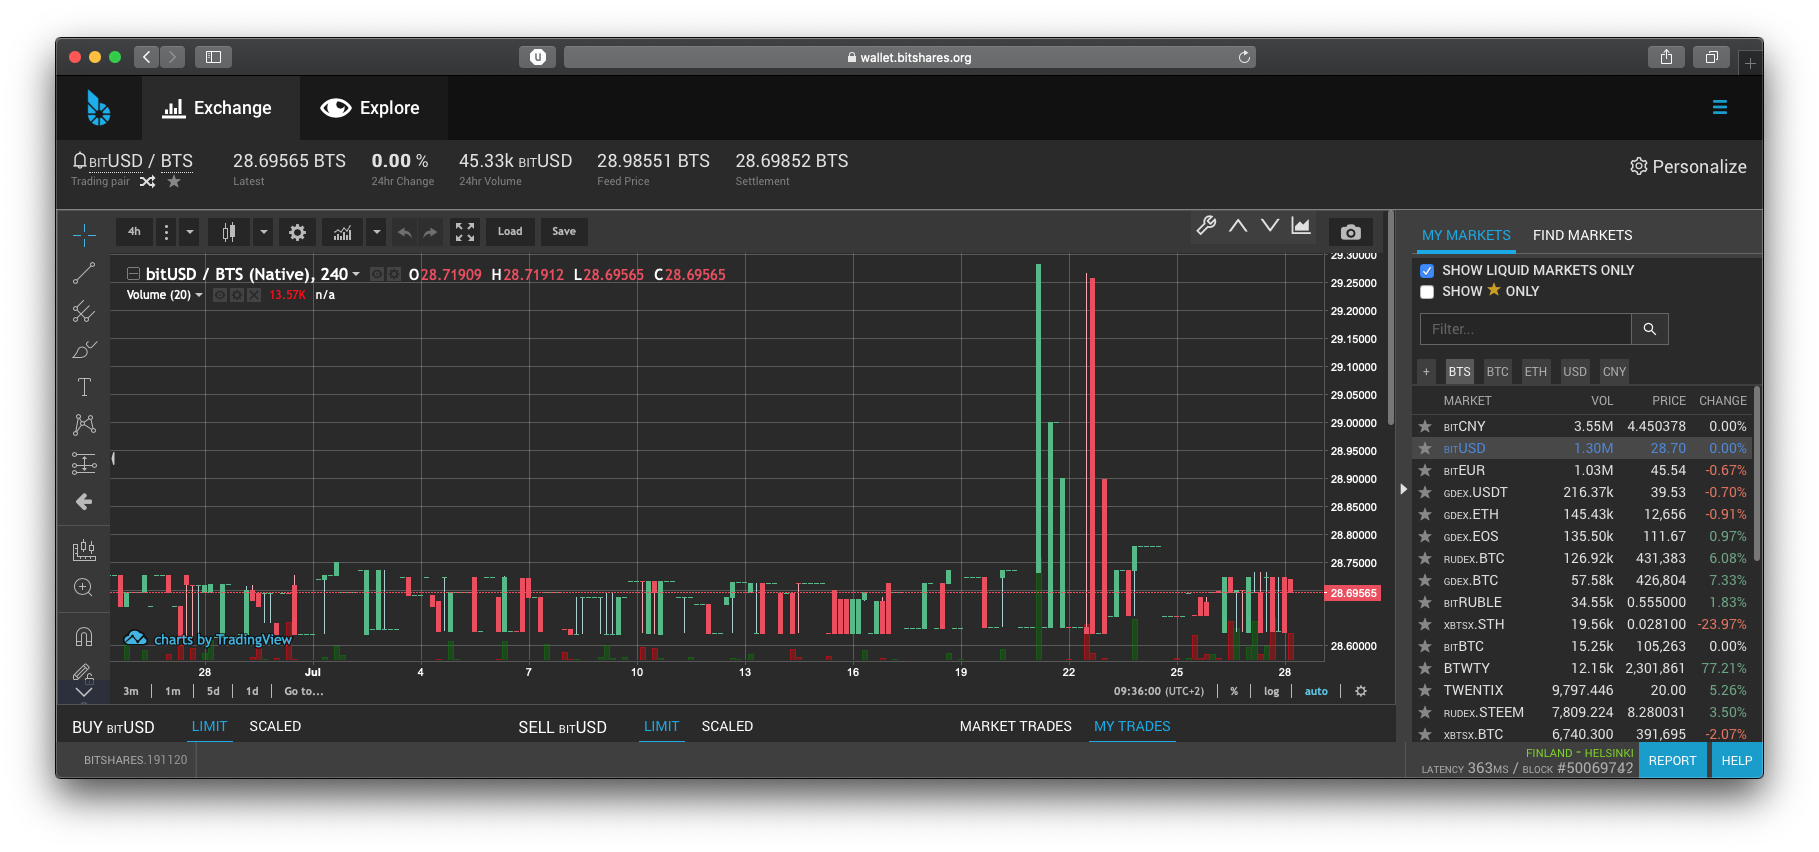
\includegraphics[width=\linewidth]{introduction/assets/bitshares}
%	\caption{An online explorer provided by the BitShares DEX, showing recent and outstanding asset orders on the BitShares blockchain.}
%	\label{fig:bitshares_explorer}
%\end{figure}

\subsection{Decentralized Cryptocurrency Exchanges}
Blockchain technology is increasingly being used to build decentralized exchanges, also called \emph{DEXes}, to trade cryptocurrencies.
DEXes enable direct peer-to-peer trading without a market operator.
On DEXes, users can create their own assets, transfer owned assets to others, and trade assets with other users by publishing buy and sell orders on the blockchain.
These orders are then automatically matched by miners during the validation of new transactions.
Usually, a DEX only allows the trading of assets residing on the same blockchain.
As we will further elaborate in Section~\ref{sec:matchmaking}, order matchmaking can also proceed outside the blockchain to increase efficiency.
DEXes have become a fundamental component of Decentralized Finance (DeFi), which is an experimental form finance conducted using blockchain applications~\cite{chen2020blockchain}.
One of the largest DEXes is Uniswap, processing trade worth over \$900 billion on a daily basis, at the time of writing.\footnote{See \url{https://coinmarketcap.com/rankings/exchanges/dex/}}

We identify four advantages of DEXes over centralized cryptocurrency exchanges.
First, DEXes enhance security during the trading process; a trade is usually an atomic operation, and there is minimal risk of losing funds as long as the underlying blockchain and consensus mechanism are secure.
Second, users themselves remain in control of their funds when trading on a DEX and they do not have to transfer ownership of their assets to the market operator (noncustodiality).
Third, the transaction fees associated with trading on a DEX are usually lower compared to a centralized exchange since there is no profit-driven intermediary.
Fourth, DEXes allow users to remain anonymous, whereas centralized exchanges often require the validation of one's identity for participation.

We also point out three disadvantages of DEX-based trading.
First, many DEXes currently suffer from low liquidity and trading volume, making them less attractive for long-term trading.
Second, their transaction throughput depends on the consensus model used by the underlying blockchain, which might make particular DEXes unsuitable for bulk trading.
Finally, as DEXes and blockchains are a relatively new technology, design weaknesses can lead to the loss of funds as demonstrated by a number of recent attacks on DeFi applications~\cite{gudgeon2020decentralized,qin2020attacking}.

\section{Disintermediation in Blockchain-based Markets}
In many physical and electronic marketplaces, middlemen play a key role in the matching of buyers and sellers, and in the facilitation of transactions between traders~\cite{bakos1998emerging}.
The popularity of electronic commerce and the rise of new business models has resulted in much interest to act as \emph{trusted intermediary} to benefit from their interactions~\cite{clark1999electronic}.
A well-known example of a trusted intermediary is PayPal~\cite{paypal}, a payment service provider for retailers.
Besides providing payment services, PayPal also acts as arbitrator when a dispute between a buyer and seller arises.
The ability to act as trusted intermediaries is at the core of electronic markets and their services help to ensures that a trade between a buyer and seller who might not necessarily trust each other proceeds without issues.

Despite their prominent role, trusted intermediaries increase the costs for traders since they are usually profit-driven and charge a fee for their services.
As such, there is much interest in removing trusted intermediaries from the trading process, or \emph{disintermediation}.
Disintermediation is defined by Merriam-Webster as \enquote{the elimination of an intermediary in a transaction between two parties}.
Disintermediation is very much related to the concept of decentralization, specifically, disintermediation requires decentralization as its foundation~\cite{guo2016blockchain}.
The debate around disintermediation in electronic markets dates back to the rise of the Internet itself. % is a concept that pre-dates blockchain technology.
The Internet provided infrastructure that offers users quick and convenient access to market information, therefore opening opportunities to replace traditional broker agents whose primary role was to aggregate this market information~\cite{wigand2020whatever}.
A clear example of disintermediation can be found in the book publishing market~\cite{giaglis1999disintermediation}.
Information technology enables book buyers to quickly place their order and allows authors to only print their books when there is actual demand, therefore removing the retailer from the book supply chain.

Bitcoin and subsequent blockchain-related innovations have further challenged the need for trusted intermediaries.
%For example, a financial institution acts as intermediary in traditional payment systems and handles all payments between different (possibly foreign) banks.
By leveraging cryptographic techniques, cryptocurrencies have demonstrated that a decentralized payment system without financial institutions is possible.
Since the introduction of Bitcoin, there has been much effort by both industry and academia to critically assess the necessity of trusted intermediaries, and potentially replace them with another mechanism, e.g., using smart contracts on Ethereum~\cite{lande2018sok}.

In many scenarios, it has been proven to be possible to replace trusted intermediaries with cryptographic techniques.
Yet, disintermediation is not always possible, and sometimes not even desired.
In many scenarios there is a need to safeguard certain processes by traditional trusted intermediaries, in particular in the financial sector.
One might argue that electronic markets require at the very least some trusted intermediary to act as mediator between buyer and sellers if a trade is not an atomic operation.
Furthermore, local regulations might require a trusted intermediary for certain market processes, e.g., when there is a need to verify the identify of business relations to prevent criminal activities (this process is also known as Know-your-Customer).

As also pointed out by other researchers, we argue that it is unlikely that electronic markets will be fully disintermediated by blockchain technology anytime soon~\cite{zamani2018little}.
Instead of complete disintermediation, it is a more likely scenario that the role of existing intermediaries will transform and that their involvement in market processes will be reduced.
For this reason, numerous financial institutions are currently experimenting with distributed ledger technology to make existing settlement services more efficient and reliable.
Perhaps the most influential solution, Corda, is currently being deployed by R3, a consortium consisting of the world's leading financial institutions~\cite{brown2016introducing}.
Another example is Ripple~\cite{armknecht2015ripple}, a credit network that is aimed to eventually replace the SWIFT payment infrastructure.
%In practice, these solutions are not fully disintermediated since payments will still be processed by nodes operated by the involved financial institutions.

\begin{figure}[t]
	\centering
	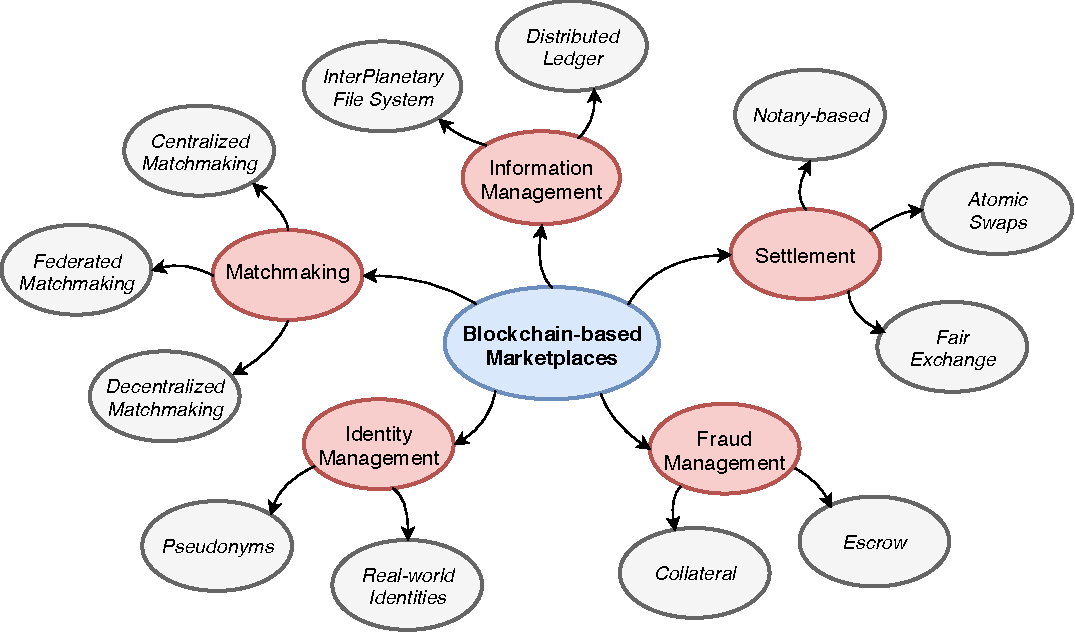
\includegraphics[width=\linewidth]{introduction/assets/decomposition}
	\caption{The five aspects of blockchain-based marketplaces (coloured in green). For each aspect, we identify existing mechanisms (coloured in grey).}
	\label{fig:electronic_markets}
\end{figure}

\section{Aspects of Blockchain-based Marketplaces}
So far, we have outlined how blockchain technology is being applied to build decentralized marketplaces and how cryptographic techniques are capable of replacing trusted intermediaries in existing electronic markets.
We now shift our focus to the aspects of blockchain-based marketplaces.
First, it is crucial to carefully define what a blockchain-based marketplace means in the context of this thesis.
We observe that there is much ambiguity around the concept of blockchain-based marketplaces in academic work.
This confusion is partially explained by the fact that electronic markets have different aspects, and blockchain technology can be applied to all or a subset of these aspects.
For example, OpenBazaar is a decentralized marketplace that leverages cryptocurrencies for peer-to-peer payments between merchants and customers but uses a traditional peer-to-peer network to share product listings amongst participants~\cite{openbazaar}.
In the context of this thesis, we define a blockchain-based marketplace as \emph{a marketplace that leverages blockchain technology to carry out one or more of its critical operations}.

We break up blockchain-based marketplaces in five different aspects.
We then assess how the concepts of decentralization and disintermediation relate to each aspect.
Figure~\ref{fig:electronic_markets} shows the five aspects of a blockchain-based marketplace, which are \emph{information management}, \emph{matchmaking}, \emph{settlement}, \emph{fraud management} and \emph{identity management}.
This figure is the result of our literature analysis, where we have studied scientific material on electronic marketplaces that leverage blockchain technology.
We decompose each aspect into commonly used mechanisms.
In the remainder of this section, we elaborate on each aspect and the existing mechanisms.

\subsection{Information Management}
Electronic markets in general require a mechanism to manage and store all market information.
This market information includes product listings, outstanding orders, and details on historical transactions (which is often used to estimate the trustworthiness of market participants).
Traditional electronic marketplaces take a centralized approach to information management and maintain all market data on their servers.
The advantage of this approach is that centralized servers are relatively straightforward to set up and maintain.
Furthermore, they enable the market operator to optimize the access to stored information by participants.
However, since the operator manages the market information, it is prone to manipulation, e.g., by tampering with or filtering search results.

Except for a few DEXes (e.g., IDEX and EtherDelta), we find that most blockchain-based marketplaces take a decentralized approach to information management and refrain from storing market information on centralized servers.
We identify two conventional approaches to data storage and dissemination of market information, which are outlined in the remainder of this subsection.

\subsubsection{Distributed Ledger}
Many blockchain-based marketplaces persist their market information on a distributed ledger, e.g., a blockchain.
In this situation, the full market state is stored within transactions on a tamper-proof distributed ledger, secured by a consensus mechanism.
New users interested in the current market state are required to download the entire distributed ledger from the network.
Since blockchain is an append-only data structure, no information is ever removed from the distributed ledger.
Therefore, some blockchains have relatively high storage requirements, for example, the entire Bitcoin blockchain requires around 290GB of storage at the time of writing.\footnote{https://www.blockchain.com/charts/blocks-size}
Some blockchain-based marketplaces deploy one or more \emph{full nodes} that remain synchronized with the network and can be queried by market participants.
These full nodes ensure quick bootstrapping in the network.

\subsubsection{Distributed Filesystem}
The high costs associated with storing data on a blockchain has motivated some blockchain-based marketplaces to leverage another storage mechanism besides a distributed ledger.
Distributed file systems have proven to be a robust solution for the storage of binary data across a network.
There is a wide range of research on using Distributed Hash Tables (DHTs) for the structured storage of key-value pairs~\cite{maymounkov2002kademlia}.
PeerMart, a decentralized marketplace for trading of Internet resources, leverages a DHT to store pricing information on offered resources~\cite{hausheer2006peermart}.

The InterPlanetary File System (IPFS) is a decentralized peer-to-peer network for the storage of and access to files, websites, applications, and data~\cite{benet2014ipfs}.
IPFS builds on top of libp2p~\cite{benet2018libp2p}, a networking framework created for decentralized protocols.
OpenBazaar, one of the most popular decentralized marketplaces, builds on IPFS to store and share market information~\cite{openbazaar}.
FileCoin, a decentralized market for file storage, also leverages IPFS to store market data~\cite{benet2018filecoin}.
%A common market type is a financial exchange where financial instruments like currencies or bonds are being traded.
%The buy and sell orders in these markets are usually bundled in an \emph{order book}.
%An order book lists the specific assets or services that are being bought or sold within a market.
%It provides traders with a convenient view on the current supply and demand.
%Depending on the market and assets being traded, the order book sometimes reveals the identity of a trader behind an open order, or their reputation scores (for instance, Airbnb shows the reputation of hosts).
%When presenting an order book to traders, ask and bid orders are usually sorted, i.e. based on their price.
%For orders with a price, ask orders are sorted ascending on price in the order book and bid orders descending on price (the best orders are presented first).
%Market orders rarely end up in the order book as open order, since they are often fulfilled instantly.
%A defining metric used by traders is the difference between the price of the highest ask order and the price of the lowest bid order, also called the \emph{bid-ask spread}.
%For the order book shown in Figure \ref{fig:order_book}, the bid-ask spread is \$149.57 - \$149.54 = \$0.03.
%This metric also indicates market liquidity, the degree to which assets can be quickly bought or sold.
%A liquid market is often characterized by a low bid-ask spread.
%The set of all ask or bid orders at a specific price is called a \emph{price level}.

\begin{figure*}[t]
	\centering
	\begin{subfigure}[t]{.33\textwidth}
		\centering
		\captionsetup{width=.9\linewidth}
		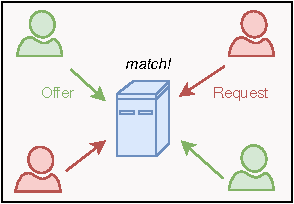
\includegraphics[width=.9\linewidth]{introduction/assets/centralized_matchmaking}
		\caption{\emph{Centralized matchmaking}: a new order is always sent to a single matchmaker.}
		\label{fig:centralized_matchmaking}
	\end{subfigure}%
	\begin{subfigure}[t]{.33\textwidth}
		\centering
		\captionsetup{width=.9\linewidth}
		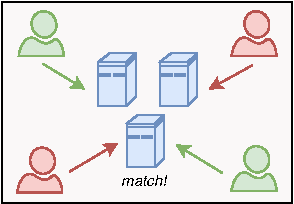
\includegraphics[width=.9\linewidth]{introduction/assets/federated_matchmaking}
		\caption{\emph{Federated matchmaking}: a new order is sent to one of the available matchmakers.}
		\label{fig:federated_matchmaking}
	\end{subfigure}%
	\begin{subfigure}[t]{.33\textwidth}
		\centering
		\captionsetup{width=.9\linewidth}
		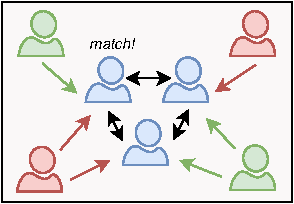
\includegraphics[width=.9\linewidth]{introduction/assets/decentralized_matchmaking}
		\caption{\emph{Decentralized matchmaking} a new order is sent to multiple matchmakers.}
		\label{fig:decentralized_matchmaking}
	\end{subfigure}
	\caption{Three approaches for matchmaking. Traders create offers and requests (coloured green and red respectively), which are matched by matchmakers (depicted in blue).}
	\label{fig:matching_architectures}
\end{figure*}

\subsection{Matchmaking}
\label{sec:matchmaking}
\emph{Matchmaking} between buyers and sellers is a prerequisite for online trade and therefore essential for any marketplace.
Matchmaking is defined as the process of mediating supply and demand in markets, based on profile information~\cite{veit2003matchmaking}.\footnote{In multi-agent systems, a matchmaker is considered as an entity that only aggregates offers. Brokers aggregate both offers and requests. We will use the term matchmaker in this thesis since we found it to be more common in related work.}
Matchmaking depends on the individual constraints and preferences of market participants.
Notable examples are the matching of idle agents to incoming jobs or the matching of suppliers of specific assets to buyers with interest in these assets.
Inefficient matchmaking between participants decreases overall market efficiency and customer satisfaction~\cite{Wu2015TheM}.
For example, prolonged suboptimal matching in a ride-hailing market like Uber increases the waiting time for passengers and forces drivers to traverse a greater distance to pick up their customers.

In many blockchain-based markets, a trader includes its buy or sell intentions in an \emph{order} that indicates their intention to buy and sell assets, resources, or services~\cite{veit2003matchmaking}.
This order is then sent to one or more matchmakers.
In general, the economic literature distinguishes between two types of orders: \emph{offers}, created by traders offering a specific asset, service, or resource, and \emph{requests}, created by interested buyers.
The main objective of a matchmaker is a quick and effective mediation between incoming offers and requests, based on the constraints and preferences included in each order.
Matchmakers match incoming offers and requests with other requests and offers, respectively, according to a \emph{matching policy}.

In Figure~\ref{fig:matching_architectures} we show three approaches for matchmaking: \emph{centralized matchmaking}, \emph{federated matchmaking}, and \emph{decentralized matchmaking}.
We now elaborate on each approach.

\subsubsection{Centralized Matchmaking}
Centralized matchmaking (Figure~\ref{fig:centralized_matchmaking}) is the most common solution to match market orders.
Traders send new offers and requests to a dedicated matchmaker, usually a centralized system (server).
This model is widely adopted by commercialized marketplaces such as stock exchanges (e.g., NYSE or NASDAQ) and resource-sharing markets (e.g., Uber and AirBnb).
Note that centralized matchmaking can be implemented with a replicated system architecture, to ensure fault tolerance and availability.

Centralized matchmaking with a single server is relatively straightforward to implement since all network communication follows the client-server model, i.e., there is no synchronization required between peers.
Also, since all orders are stored and matched by a single matchmaker, orders can be processed based on full market knowledge and therefore matched optimally with existing orders.
With centralized matchmaking, the identity behind each order is only disclosed to the market operator, therefore protecting the privacy of individual traders.

The emergence of electronic trading, in general, gave rise to fairness, transparency and manipulation issues during the matchmaking process~\cite{mavroudis2019libra}.
For example, with centralized matchmaking, the matchmaker is capable of censoring or delaying specific orders.
Information asymmetry between market operators and traders allows matchmakers to exploit their information advantage, e.g., by front-running on specific orders.
From a systems perspective, centralized matchmaking has lower scalability compared to distributed solutions since the matchmaker becomes a bottleneck when more orders are being submitted within the same period.
Finally, centralized matchmaking exhibits low fault tolerance: if the single matchmaker becomes unavailable, e.g., due to infrastructure failures, incoming orders cannot be matched and all market activity stalls.

Within the context of blockchain-based marketplaces we find that centralized matchmaking is widely adopted by centralized cryptocurrency exchanges.
For DEXes, this model is uncommon since matchmaking can proceed as part of the blockchain logic.
Notable exceptions are the Ethereum-based exchanges EtherDelta~\cite{etherdelta} and IDEX~\cite{idex} that deploy one or more servers to store and match market orders.

%EtherDelta maintains a single server that stores an order book with all active orders.
%Traders can browse the order book and trade against orders in the order book.
%The trades are finalized on the blockchain, and the order is then removed from the EtherDelta order book.\todo{custodial vs non-custodial}
%The IDEX exchange also deploys a centralized server but automatically matches orders submitted by makers and takers~\cite{AuroraLabs:B4jmyRY8}.
%Specifically, traders lock their assets in the IDEX smart contract and submit their order to the IDEX server, which checks its validity.
%The order is then executed by the Ethereum smart contract and the order book is updated according to the executed trade.

\subsubsection{Federated Matchmaking}
%Figure \ref{fig:federated_matchmaking} illustrates an alternative model for order matching: federated matchmaking.

Federated matchmaking (Figure~\ref{fig:federated_matchmaking}) is an alternative approach where instead of relying on a central matchmaker, multiple (independent) matchmakers individually maintain an order book.
The set of matchmakers can either be static, e.g., elected by a committee or some voting mechanism, or dynamic, e.g., each peer can opt-in to become a matchmaker for others.
A new order is submitted to one of the available matchmakers, selected by the order creator.
The reliability or trustworthiness of individual matchmakers might impact the choice for the preferred matchmaker.
When a matchmaker is suspected of mistreating incoming orders, or when the matchmaker is unreliable, traders can entrust their orders to another matchmaker instead.
This approach increases robustness against failure of individual matchmakers since a trader can send its order to another available matchmaker in this situation.
However, the market orders are fragmented now across different matchmakers, potentially leading to sub-optimal market efficiency compared to centralized matchmaking.

%Blockchain-powered marketplaces based on the 0x and AirSwap protocols have adopted the federated matchmaking model~\cite{warren20170x}~\cite{oved2017swap}.
%The 0x protocol uses off-chain order relaying and on-chain settlement, meaning that orders are created shared, and matched outside a blockchain.
%A maker creates market liquidity in 0x by first selecting an available relayer.
%Each relayer maintains an off-chain order book and charges a transaction fee for its services.
%The maker then creates the order and specifies a fee which is given by the selected relayer.
%Takers query the order book of relayers and if they intend to fulfill an order, they submit it to the Ethereum blockchain.
%The Augur prediction market (see Section~\ref{sec:prediction_markets}) leverages the 0x protocol for order dissemination and matching.

%The Swap protocol follows a similar off-chain matchmaking, on-chain settlement model~\cite{oved2017swap}.
%In Swap, indexers aggregate trade intents created by market makers and takers.
%The indexer informs takers when a matching trade intent has been found, upon which a peer-to-peer negotiation process starts between the matched maker and taker.
%During this negotation process, a maker may contact an oracle to get a price suggestion.
%When a maker and taker agree on a trade, the taker submits the agreement to an Ethereum smart contract, upon which the trade is executed and on-chain assets are exchanged.
%We remark that both 0x and Swap are limited to trading Ethereum-based digital tokens and can therefore not be used for order processing of any blockchain-based asset.

%Federated matchmaking allows traders to select their preferred matchmaker.

The 0x~\cite{0x} and Swap trading protocols, enabling the trade of Ethereum tokens, have adopted the federated matchmaking model.
Both protocols allow any user to act as matchmaker and therefore build an off-chain matchmaking network for orders.
We observe, however, that the most used matchmaker is often the one provided by the protocol developers.
This makes the added benefit of this approach, compared to centralized matchmaking, questionable.

\subsubsection{Decentralized Matchmaking}
The main idea of \emph{decentralized matchmaking} is that a single order is sent to multiple matchmakers simultaneously.
In addition, matchmakers are able to synchronize known orders with other matchmakers.

This approach is exclusively used in the context of blockchain-based marketplaces, to the best knowledge of the authors.
Most DEXes that operate on a blockchain use \emph{on-chain} decentralized matchmaking.
This process either relies on a smart contract to match known orders or executes the matchmaking logic as part of the transaction validation.
The market orders are embedded in transactions and sent to miners for inclusion on the blockchain.
For example, Stellar maintains an exchange on its distributed ledger and allows users to issue buy and sell orders for any asset that is native to the Stellar blockchain~\cite{lokhava2019fast}.
In the same way, the BitShares DEX offers specialized transactions to create new or cancel existing orders~\cite{schuh2015bitshares}.

The main advantage of on-chain decentralized matchmaking is tight integration with the blockchain logic; no additional components are required to process and match orders.
However, since users need to pay fees when creating the transactions to manage their orders, order management can become costly, in particular when done in bulk.
Furthermore, matching on a blockchain can be orders of magnitude slower compared to centralized matchmaking, due to the need to reach a network-wide consensus on all transactions.
Finally, on-chain matching protocols do not explicitly store all established matches.
Therefore, to reconstruct the order book at a specific block height, one needs to replay all transactions up to that block in the blockchain.

Some blockchain-based marketplaces maintain the order book \emph{off-chain} to lower the costs of order management.
Loopring, for example, is an order sharing protocol where new orders are sent to one or more relays in an off-chain mesh network~\cite{loopring}.
Relayers claim the margin between two matched orders, or can alternatively charge a fixed fee for their services.
The Republic Protocol builds a decentralized network of nodes that match orders without revealing any information about individual orders~\cite{zhang2017republic}.
The protocol uses Shamir secret sharing~\cite{shamir1979share} to break down an order in multiple order fragments which are distributed through the network, thus hiding the identity of the order creator.
%Loopring is able to mix and match multiple orders in circular trade, also called order rings, therefore increasing liquidity.
%Order rings are submitted to a smart contract, e.g., on Ethereum, where the trade is then executed.
%Relayers can optionally share orders with other relayers to increase liquidity, however, the whitepaper lacks technical details on how this is achieved specifically.

% front-running in Loopring

%An Ethereum smart contract, called the Registrar, describes the network topology such that it is hard for an adversary to fully reconstruct an original order.
%Nodes cooperate with other nodes to check if their order fragments match, by computing a zero-knowledge proof.
%When two order fragment match, an atomic swap is initiated between the two traders (also see Section~\ref{sec:atomic_swap}).
%Note that this prevents an individual from estimating the total liquidity in the network.

We identify two advantages of decentralized off-chain matchmaking compared to centralized and federated matchmaking.
First, by sharing orders between matchmakers, one can achieve similar matching effectiveness compared to centralized matchmaking, depending on how quickly orders are synchronized amongst matchmakers.
Second, decentralized matchmaking exhibits high tolerance against the failure of individual matchmakers and can withstand the failure or partition of a subset of all matchmakers.
However, this model increases bandwidth usage since orders are replicated over multiple matchmakers.
It also might take longer before a new order is fulfilled in the case that it is sent to matchmakers that are unable to match this order immediately.

\subsection{Settlement}
Secure trade \emph{settlement} in blockchain-based marketplaces is a difficult research challenge.
%After two parties have agreed to trade, a value exchange must take place.
Settlement is the process of fulfilling the obligations by trading parties.
In traditional marketplaces and many cryptocurrency exchanges, it is common practice to have a trusted intermediary settle a trade.
A trade using a trusted intermediary completes as follows: two parties that agree on a trade transfer the assets for sale to one of the wallets owned by the trusted intermediary.
When this intermediary has received both assets, it finishes the exchange by transferring the appropriate assets to the other party.
In this approach, the trusted intermediary holds (temporary) ownership of the assets to be traded.
Relying on a trusted intermediary removes the risks when trading directly between the parties, but it requires both parties to have faith that the intermediary does not default or steal their assets.

%Trade through a trusted intermediary can facilitate value exchange between an extensive range of different blockchains, as long as the intermediary maintains wallets on the involved blockchains and can issue transactions in these systems to transfer the assets.
%This is usually not an issue in permissionless blockchains since anyone can create accounts or wallets by generating a new cryptographic key pair.
%Centralized cryptocurrency exchanges often facilitate asset trading across numerous permissionless blockchains.
%Some cryptocurrency exchanges process transactions worth millions of dollars in total daily.\footnote{See https://coinmarketcap.com/rankings/exchanges}
%In a permissioned blockchain environment, however, a trusted intermediary coordinating an asset exchange requires explicit approval from the operator to read and write transactions on the involved distributed ledgers.
%Allowing new parties in a permissioned blockchain might be undesirable by operators since it introduces additional legal and operational risks.

Blockchain-based marketplaces refrain from settlement through a trusted intermediary and either use cryptographic techniques to ensure atomicity, or rely on a group of semi-trusted peers to settle a trade.
We outline three settlement techniques commonly found in blockchain-based marketplaces.

\begin{figure}[t]
	\centering
	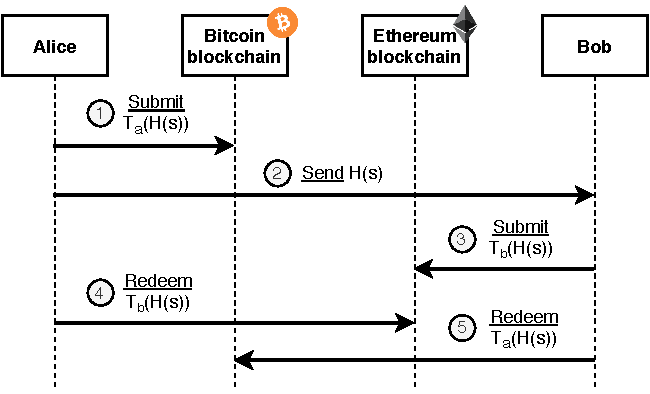
\includegraphics[width=.7\linewidth]{introduction/assets/atomic_swap}
	\caption{Sequence diagram of a successful HTLC-based atomic swap between Alice and Bob.}
	\label{fig:atomic_swap_intro}
\end{figure}

\subsubsection{Atomic Swaps}
The \emph{atomic swap} is a protocol that is commonly used to exchange assets between different blockchains, without need for a trusted intermediary~\cite{herlihy2018atomic}.
Atomic swaps enable two parties to exchange blockchain-based assets in an atomic manner.
This means that the exchange either completes for both parties and have their assets traded, or it fails.
When the exchange fails, both parties do not suffer an economic loss and retain ownership of the assets involved in the exchange.
We remark that the atomicity property of the atomic swap protocol critically depends on the characteristics of the underlying blockchains.
If one of the blockchains is compromised by adversaries, or if a chain reorganization occurs, atomicity during asset exchange cannot be guaranteed and one of the parties can lose its funds to the counterparty.

Atomic swaps eliminate the risk of losing assets to an adversarial trader during the exchange.
The main idea is that trading users lock their assets in a specialized transaction on the blockchain in such a way that no single party can claim both locked assets.
This is achieved with \emph{Hash-Timelock Contracts} (HTLCs), a special transaction that leverages hash locks and time locks.
A hash lock is a restriction that prevents the transfer of assets until the pre-image of a provided hash is revealed.
A time lock is a primitive that locks assets until a specific time.
They prevent the assets being traded from being locked up indefinitely during an atomic swap.
This time lock should be well above the block confirmation time of the underlying blockchain to prevent the loss of assets during a blockchain reorganization.
In practice, this value is often fixed to several hours.

We further explain the atomic swap by considering a trade with Bitcoin and Ether (the native token of the Ethereum blockchain).
Figure~\ref{fig:atomic_swap_intro} visualizes an atomic swap between two parties, Alice and Bob, where Alice sells her Bitcoin in return for Ether.
The basic atomic swap, described by Tier Nolan~\cite{nolan2016atomic}, consists of the following six steps:

\textbf{Step 1.} Alice generates a secret value $ s $ and computes $ H(s) $, where $ H(\cdot) $ is a secure hash function.

\textbf{Step 2.} Alice submits a hash-timelock transaction $ T_1 $ to the Bitcoin blockchain, locking her Bitcoin and using $ H(s) $ for the hash lock. A party can claim the Bitcoin held by $ T_1 $ with another transaction that provides $ s $, within a specific time duration.

\textbf{Step 3.} Alice sends $ H(s) $ to Bob using any communication medium.

\textbf{Step 4.} Bob submits a hash-timelock transaction $ T_2 $ to the Ethereum blockchain, locking his Ether and also using $ H(s) $ for the hash lock.

\textbf{Step 5.} Alice claims the Bobs' Ether locked in $ T_2 $ by submitting a transaction, $ T_3 $, to the Ethereum blockchain, containing $ s $. $ T_3 $ unlocks the hash-lock in $ T_2 $. This reveals pre-image $ s $ to Bob.

\textbf{Step 6.} Bob now claims Alice's Bitcoin locked in $ T_1 $ by submitting a transaction, $ T_4 $, to the Bitcoin blockchain, containing $ s $. The asset exchange is now complete.

The above protocol requires a total of four transactions.
Note how Alice is not able to claim assets without providing the opportunity for Bob to claim her assets.

%First, Alice generates a random secret $ s $ and computes $ H(s) $, where $ H(\cdot) $ denotes a hash function.
%She then submits a hash-locked transaction, indicated by $ T_a(H(s)) $ (step \circled{1}), to the Bitcoin blockchain that transfers her Bitcoin to Bob's wallet address.
%A hash-locked transaction is only executed when the secret $ s $ is provided to it.
%Alice now sends $ H(s) $ to Bob (step \circled{2}).
%Bob then submits a transaction $ T_b(H(s)) $ with the same hash lock to the Ethereum blockchain, transferring his Ethereum to the account of Alice (step \circled{3}).
%Alice is now able to claim the assets held in custody by $ T_b(H(s)) $ (since she knows the value of $ s $), which in turn reveals $ s $ to Bob (step \circled{4}).
%Bob now completes the swap by submitting $ s $ to the $ T_a(H(s)) $ transaction on the Bitcoin blockchain, which unlocks the assets in $ T_a(H(s)) $ (step \circled{5}).
%To prevent the situation where assets are locked indefinitely if Alice refuses to reveal $ s $, Alice and Bob submit two additional time-locked transactions to ensure that assets in $ T_a(H(s)) $, respectively $ T_b(H(s)) $, can be claimed after some time $ t_1 $, respectively $ t_2 $.
%To address the situation where Alice claims the assets in both $ T_a(H(s)) $ and $ T_b(H(s)) $, it must hold that $ t_1 > t_2 $.
%These hash- and time-based agreements, also called Hashed Timelock Contracts (HTLCs), thus ensure trust-less, atomic asset exchange between trading parties, assuming that they claim the assets before the time-lock expires.

\subsubsection{Fair Exchange}
Fair exchange is a well-studied technique in computer science and is leveraged by a few blockchain-based marketplaces as settlement mechanism~\cite{pagnia2003fair}.
An exchange is considered fair if both of the parties receive the items they expect, or none of them do.
Therefore, the atomic swap can be considered as a class of fair exchange protocols.
The FairSwap protocol ensures a fair exchange of digital goods by leveraging smart contracts and zero-knowledge proofs~\cite{dziembowski2018fairswap}.
The protocol, however, is designed around the exchange of digital commodities and is therefore not usable for generic asset exchange across different blockchains.
Optimistic fair exchange algorithms address counterparty risk by relying on the arbitration by a trusted third party when one of the involved traders attempts to cheat~\cite{asokan1997optimistic}.
Optimistic fair exchange has been initially applied for the exchange of digital signatures but has recently been leveraged to ensure the execution of a cryptocurrency payment in exchange for a receipt~\cite{liu2018toward}.
This class of algorithms, however, requires the participation of a trusted third party to resolve disputes.

\subsubsection{Notary-based}
Notary-based schemes are another approach to trade settlement where the approval by a group of credible nodes (often called notaries) is required to perform some operation.
Notary schemes aim to partially alleviate the trust issues arising when relying on a single trusted intermediary through the approval by a group of semi-trusted notaries instead.
These notaries reach consensus on the occurrence of particular events, e.g., on the inclusion of a transaction on a distributed ledger.
Compared to an asset exchange through a trusted intermediary, notary schemes assume a weaker trust model compared to settlement with a trusted intermediary. Furthermore, they can usually withstand adversarial behaviour of a fraction of all notaries.

The Interledger project, pioneered by Ripple, is the most advanced approach in this direction~\cite{thomas2015protocol}.
Interledger proposes a notary-based protocol to conduct payments across different ledgers.
In atomic mode, these payments are realized through atomic swaps and are coordinated by a different group of notaries for every involved blockchain.
Interledger uses payment paths where additional intermediate platforms and their notaries are used to exchange assets between ledgers that do not have a direct connection.
Interledger also supports bidirectional asset exchange but is vulnerable to a fraction of notaries colluding with one of the trading parties.
%External coordination is avoided in universal mode, which relies on incentives for participants to behave honestly and not to commit fraud.

\subsection{Fraud Management}
The management of fraud is a crucial challenge in any marketplace and is closely related to the settlement process.
The risk of fraud typically occurs when a buyer and seller have never interacted before and therefore do not have a prior trust relation.
A common type of fraud is \emph{counterparty fraud}, where a party does not fulfil its obligation towards the counterparty during the settlement of a trade, e.g., by not delivering the promised assets or goods.
In centralized marketplaces, this kind of fraud is often resolved by the market operator, acting as arbitrator during the dispute resolution process.
Within blockchain-based marketplaces, however, counterparty fraud is often prevented since blockchain transactions are atomic: either both trading parties receive their assets, or nothing happens.
%This approach works when assets can be exchanged directly, e.g., on a blockchain-powered DEX.
Fraud management, however, becomes instrumental when the settlement process is not atomic and requires both involved traders to move value to the counterparty manually. % depends on the actions of users.
We identify two conventional approaches to manage fraud arising during a non-atomic trade in blockchain-based marketplaces: using escrow services and collateral.

\subsubsection{Escrows}
Some blockchain-based marketplaces are using a third-party escrow service when a dispute arises.
This escrow may be a single entity, e.g., another user in the marketplace, or a group of users with some authority to resolve the dispute.
In the Bisq decentralized exchange, for example, users can make a call on mediators or arbitrators to resolve fraud~\cite{bisq}.
Mediators attempt to resolve the dispute but do not have authority over the funds being traded.
Arbitrators, however, can redistribute traded assets through the usage of multi-signature techniques.

\subsubsection{Collateral}
Some blockchain-based marketplaces require users to deposit collateral before trading.
This collateral is slashed when its depositor does not adhere to an agreement or deviates from the protocol.
The XClaim protocol, for example, relies on collateral deposits to enable asset trading between distinct blockchain ledgers and to incentivize users to behave in line with the system rules~\cite{zamyatin2019xclaim}.
When a participant misbehaves, the collateral is slashed, and wronged actors are reimbursed.

\subsection{Identity Management}
The final research challenge we identified in blockchain-based marketplaces is how to manage the digital identities of participants.
Traders enter a blockchain-based marketplace under a digital identity.
We discuss two approaches to identity management in blockchain-based marketplaces: using pseudonyms and using real-world identities.

\subsubsection{Pseudonyms}
A key property of blockchain technology is the ability to join the network under a pseudonym, a disguised identity usually in the form of a cryptographic keypair.
Users are then identified by their public key, and ensure authenticity of their transactions by signing the transactions with their private key.
Since trading on a specific DEXes is usually contained within a single market environment, DEXes do not require identity verifications and allow traders to join the network under a pseudonym.

\subsubsection{Real-world Identities}
% -> becomes required when inteacting with fiat money
In traditional electronic marketplaces, the identity under which a user operates is usually linked to a real-world identity~\cite{subramanian2017decentralized}.
Identity validation in electronic marketplaces has several purposes.
First, it ensures accountability of one's actions within the market in case of a dispute between a buyer and seller.
Second, it prevents the situation where a user can easily re-enter the market under a different identity after having committed fraud.
Third, identity verification is often part of the regulatory compliance of market operators, as often required by anti-money laundering policies imposed by governments.
For example, eBay requires its users to go through an identity verification process before they can buy or sell goods on the platform.
Similarly, some blockchain-based markets enable the trade of fiat currency for cryptocurrencies, e.g., Bisq~\cite{bisq}.
In addition, many centralized cryptocurrency exchanges require user verification since these exchanges often allow payments with fiat money.
%Although not within the scope of this thesis, it is worth mentioning how blockchain technology offers new insights on digital identities.

\section{Research Questions}
\label{sec:research_questions}
In this thesis, we focus on decentralization and disintermediation of the five identified aspects of blockchain-based marketplaces.
The overarching research question of this thesis is as follows:\\\\
\emph{How can all aspects of blockchain-based markets be decentralized and disintermediated?}\\\\
To answer our research question, we address the following five questions:

\textbf{[RQ1] How can a scalable and decentralized mechanism for the storage and dissemination of market information be built?}
Adequate management of information is essential for electronic marketplaces.
Traditional marketplace store all market orders and product listings on a (centralized) server, which is prone to manipulation by the market operator.
Blockchain-powered decentralized exchanges persist all market information on a distributed ledger but this approach suffers from scalability limitations.
Our goal is to build a scalable storage mechanism in which participants themselves manage all market information.

\textbf{[RQ2] How can market orders efficiently and fairly be matched without a centralized matchmaker?}
Order matchmaking in electronic markets is predominantly performed on a centralized server, owned by the market operator.
This approach, however, enables the operator to delay, hide, or prioritize incoming orders, resulting in an unfair system.
Leveraging blockchain technology to perform order matchmaking has the potential to address these fairness issues but is not scalable enough for usage by many marketplaces.
%Additionally, there is a lack of research on off-chain decentralized matchmaking.
We aim for an efficient matchmaking mechanism with fairness guarantees while avoiding centralized coordination by a market operator.

\textbf{[RQ3] How can the settlement durations of (international) bank payments be reduced?}
Secure settlement of a trade is a key requirement for electronic marketplaces.
Trade often involves real-world currencies that are managed by a bank.
A major problem of current banking systems is that the settlement duration of a payment between two different (international) banks is significant and can take days to complete.
Furthermore, these payments often require significant transaction fees to cover back-office costs.
%Leveraging the ideas of blockchain technology holds the potential to improve the speed of (international) payment infrastructures, and potentially leads to cost reductions.
Our goal is to reduce the settlement duration of international payments between banks.

\textbf{[RQ4] How can assets securely be exchanged between any permissioned blockchain without a trusted intermediary?}
Permissioned blockchains are gaining popularity to manage real-world asset within industrial domains such as supply chain management.
While the number of permissioned blockchains is proliferating, there is no universal mechanism to quickly exchange assets between different ecosystems without using a trusted intermediary.
%A key issue, however, is that the assets on a specific DEX are locked to a single blockchain; trade between different DEXes is either impossible, slow, or requires significant changes to deployed blockchain logic.
We aim for a universal settlement mechanism that is capable of securely exchanging assets between any permissioned blockchain.
%The question is how to address these issues and enable fast asset trading between different exchanges.

\textbf{[RQ5] How can blockchain technology be applied to build a decentralized identity for software developers?}
The engineering of blockchain-based applications is a challenging task and requires engineers with appropriate qualifications.
At the same time, the credentials of software developers are fragmented across many platforms, and vendor-locked.
This makes it challenging to get a representative impression of ones skills, e.g., as required in crowdsourcing marketplaces.
Our goal is to devise a solution to unify these credentials without data storage by a centralized provider.

%Crowdsourcing is a relatively new model for software development, where an open call is made for the documentation, design, coding, and testing of software.
%Recent research proposes to leverage blockchain technology to disintermediate in these markets.
%However, the proposed solutions are not generic and there are remaining issues regarding settlement using different currencies, and the storage of information.

\begin{table*}[t]
	\small
	\centering
	\begin{tabular}{ |c|c|c|c| }
		\hline
		\textbf{RQ} & \textbf{Mechanism} & \textbf{Experiments} & \textbf{Deployment} \\ \hline
		1 & \TrustChain{} & DAS5 + simulations & integration in Tribler \\ \hline
		2 & MATCH & DAS5 & integration in Tribler \\ \hline
		3 & XChange & DAS5 + simulations & integration in Tribler \\ \hline
		4 & Internet-of-Money & DAS5 & in-house testing \\ \hline
		5 & DevID & - & user trial \\ \hline
	\end{tabular}
	\caption{An overview of research methods for each mechanism introduced in this thesis.}
	\label{table:research_methodology}
\end{table*}

\section{Research and Engineering Methodology}
%Our work is inspired by the limitations of blockchain technology.
Blockchain is a relatively young technology of which research is conducted in economics, computer science and social sciences.
We identify two main research approaches in this field.
On the one hand, published blockchain research in systems-oriented conferences adopts experimental methods where the performance of proposed mechanisms is evaluated using a comprehensive set of experiments and benchmarks.
On the other hand, there is a vast body of theoretical research on the security aspects of distributed ledgers and their consensus algorithms.
This body of research tends to follow a theoretical approach through bound analysis, formal proofs or protocol simulations.

In this thesis, we adopt an experimental approach where we answer each research question by designing, implementing and evaluating a decentralized mechanism that targets different aspects of blockchain-based marketplaces.
%We then systematically evaluate the appropriate properties of each mechanism (e.g., scalability), and if feasible, we deploy our mechanisms to users to analyse our system in a real-world environment.
For all of our proposed mechanisms, our primary objective is to build a solution that is ready for deployment and usable by end users.
We have implemented each mechanism in the Python programming language, usually within a few thousand lines of code.
We utilize an existing library for networking primitives, fully developed by our lab.\footnote{See \url{https://github.com/tribler/py-ipv8}}
Table~\ref{table:research_methodology} lists for each mechanism how we have evaluated and deployed it.
Except for DevID, we evaluate each mechanism with an appropriate set of experiments using our nation-wide compute cluster (the DAS5~\cite{bal2016medium}).
We have also evaluated the \TrustChain{} and XChange using simulations.
These simulations enables us to evaluate a mechanism with many users and allows us to quickly replay longitudinal real-world traces (e.g., we evaluate the XChange mechanism by replaying a week of buy and sell orders).

Driven by our focus on practicality, we have deployed each mechanism proposed in this thesis, either to a small group of colleagues or with an integration in the Tribler application~\cite{zeilemaker2011tribler}.
Tribler is our open-source, academic research vehicle and offers decentralized, anonymous file-sharing capabilities.
Tribler has been downloaded by over 1.5 million users and enables us to test our ideas and code in a geo-distributed, real-world environment and on consumer-grade hardware.
For example, we have integrated \TrustChain{} in \Tribler{} to prevent free-riding behaviour in our anonymous peer-to-peer overlay.
This two-year deployment period of \TrustChain{} has allowed us to incrementally improve our accounting mechanism and refine our ideas.
We attempt to make our research reproducible by publishing the implementation of each mechanism, including documentation and unit tests, on GitHub.\footnote{Links to the implementation are provided in the remaining chapters of this thesis.}
Due to legal considerations, we are unable to provide an open-source implementation of the four reverse-engineered banking algorithms associated with our Internet-of-Money mechanism.

The complexity of real-world systems often posed a challenge when deploying our mechanisms.
For example, shortly after the initial deployment of the MATCH mechanism in \Tribler{} (see Chapter~\ref{chapter:match}), students forged a specific packet that would crash a Tribler instance that received it.
Tribler would forward the packet to other connected peers before crashing.
Therefore, this bug affected a large part of our network and we were forced to deployed a fix for this behaviour by releasing a new version of Tribler.
Despite the large efforts required to get a system deployed and operational, this process has been tremendously helpful in discovering both critical design flaws and minor implementation errors.

%Distributed systems can be complex software implementations with many components that work together.
%Specifying the scope of a system is a non-trivial challenge and failing to implement clear system boundaries can result in numerous performance bottlenecks and degradation of user experience when such a system is deployed.
%To this end, during the design of each mechanism we specify the boundaries of each system and state what we consider out of scope.
%We aim to focus on the core functionality of each mechanism.

% simplicity?

%We believe this experimental research methodology is suitable for two reasons.
%First, it allows us to evaluate our ideas in an environment that closely resembles a real-world environment.
%Second, it directly leads to a software implementation that can be used by academia or industry.
%All developed software artefacts are available on our GitHub repository and contain unit tests to verify functional correctness.

% existing research does X

% but we do Y!

\begin{figure}[t]
	\centering
	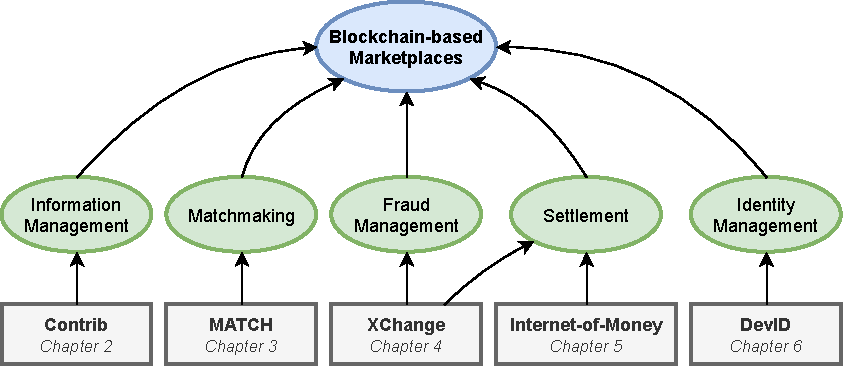
\includegraphics[width=\linewidth]{introduction/assets/thesis_overview}
	\caption{The five decentralized mechanisms presented in this thesis, in the context of blockchain-based marketplaces and the identified aspects.}
	\label{fig:thesis_overview}
\end{figure}

\section{Thesis Outline and Contributions}
In Chapter 2-6, we address the research questions stated in Section~\ref{sec:research_questions}.
Figure~\ref{fig:thesis_overview} shows the mechanisms introduced in this thesis, and visualizes the aspect(s) that each mechanism relates to.
We do note that fraud in Figure~\ref{fig:thesis_overview} specifically refers to the act of committing counterparty fraud during a trade.
The content and contributions in each chapter are as follows:\\

\textbf{[Chapter 2] ConTrib: Maintaining Fairness in Decentralized Big Tech Alternatives by Accounting Work.}
In this chapter, we address RQ1 and build a universal mechanism for the accounting of information.
%To date, there is no such accounting mechanism that is optimized to store small pieces of information in large-scale shared-resource systems.
We present \TrustChain{}, a scalable mechanism for the accounting of interactions within a decentralized network.
Each individual in \TrustChain{} maintains a \emph{personal ledger} of tamper-evident \emph{records}.
Records can point to other ones and can be agreed on by other users, resulting in a global DAG structure.
Fraud, the illegitimate modification of a record, is effectively detected since users continuously share and validate records.
We devise a system architecture with flexible validation and fraud policies.
Our evaluation reveals that \TrustChain{} is highly scalable, tolerates packet loss and exhibits relatively low fraud detection times.
To highlight the potential of \TrustChain{}, we leverage our solution for bandwidth accounting in the \Tribler{} application and successfully address free-riding behaviour.
Our two-year deployment trial has resulted in over \TrialRecords{} records, created by more than \TrialUsers{} Internet volunteers.
We make use of the accounting capabilities of \TrustChain{} for other mechanisms introduced in this thesis, namely XChange, Internet-of-Money, and DevID.
This chapter is based on the following two publications:

Martijn de Vos and Johan Pouwelse, \enquote{ConTrib: Universal and Decentralized Accounting in Shared-Resource Systems}, \emph{Distributed Infrastructure for Common Good (DICG), 2020.}\\

Martijn de Vos and Johan Pouwelse, \enquote{ConTrib: Maintaining Fairness in Decentralized Big Tech Alternatives by Accounting Work}, \emph{Computer Networks}, 2021, Elsevier.\\

\noindent We have presented an earlier version of the \TrustChain{} mechanism (named TrustChain) in the following article:\\

Pim Otte, Martijn de Vos and Johan Pouwelse, \enquote{TrustChain: A Sybil-resistant Scalable Blockchain}, \emph{Future Generation Computer Systems (FGCS), Special Issue on Cryptocurrency and Blockchain Technology}, 2020, Elsevier.\\

In contrast to our earlier article on TrustChain, the articles presenting the \TrustChain{} mechanism contain additional details on the data structure, include a full description of our fraud detection algorithm, and include the results of our two-year deployment trial within \Tribler{}.

\textbf{[Chapter 3] MATCH: A Decentralized Middleware for Fair Matchmaking in Peer-to-peer Markets.}
In this chapter, we address RQ2 and focus on matchmaking, the process of bringing market participants together based on individual preferences.
%Although numerous companies have deployed infrastructure for matchmaking, there is currently no solution that can be deployed within different trading domains.
Matchmaking is a core enabling element in peer-to-peer markets.
To date, matchmaking is predominantly performed by proprietary algorithms, fully controlled by market operators.
This raises fairness concerns as market operators effectively can hide, prioritize, or delay the orders of specific users.
Blockchain technology has been proposed as an alternative for fair matchmaking without a trusted operator but is still vulnerable to specific fairness attacks like front-running.
We present MATCH, a decentralized middleware for fair matchmaking in peer-to-peer markets.
By decoupling the dissemination of potential matches from the negotiation of trade agreements, MATCH empowers end-users to make their own educated decisions and to engage in direct negotiations with trade partners.
This approach makes MATCH highly resilient against malicious matchmakers that deviate from a specific matching policy.
We implement MATCH and show the resilience of our middleware using real-world ride-hailing and asset trading workloads.
The author of this thesis has collaborated with Georgy Ishmaev, who framed the research problem that MATCH addresses within the broader scope of socio-ethical implication of matching platforms for peer-to-peer markets.
This chapter is based on the following publication:

Martijn de Vos, Georgy Ishmaev and Johan Pouwelse, \enquote{MATCH: a Decentralised Middleware for Fair Matchmaking in Peer-to-peer Markets}, \emph{Middleware, 2020.}\\

\textbf{[Chapter 4] XChange: A Universal Mechanism for Asset Exchange between Permissioned Blockchains.}
In this chapter, we address RQ3 and present a universal mechanism for asset exchange between permissioned blockchains.
Permissioned blockchains are increasingly being used as a solution to record transactions between companies.
Several use cases that leverage permissioned blockchains focus on the representation and management of real-world assets.
Since the number of incompatible blockchains is quickly growing, there is an increasing need for a universal mechanism to exchange, or trade, digital assets between these isolated platforms.
There currently is no universal mechanism for inter-blockchain asset exchange without a requirement for trusted authorities that coordinate the trade.
We address this shortcoming and present the XChange mechanism.
To achieve universality and to avoid trusted authorities that coordinate a trade, XChange does not provide atomic guarantees but leverages risk mitigation strategies to reduce value at stake.
Our mechanism records the specifications and progression of each trade within records on a distributed log.
XChange reduces the economic gains of adversaries by bounding the total amount of fraud they can commit at any time.
After having committed fraud, an adversary is forced to finish its ongoing trades before it can engage in new trades.
We first present a four-phased protocol that coordinates an asset exchange between two traders.
We then outline how trade records can be stored on the distributed TrustChain ledger.
We implement XChange and conduct experiments.
Our experiments demonstrate that XChange is capable of reducing the economic gains of adversaries by more than 99.9\% when replaying a real-world trading dataset.
A deployment on low-resource devices reveals that the latency added to a trade by XChange is only 493 milliseconds.
Finally, our scalability evaluation shows that XChange achieves over 1’000 trades per second and that its throughput, in terms of trades per second, scales linearly with the system load.
This chapter is based on the following publication:

Martijn de Vos, Can Umut Ileri and Johan Pouwelse, \enquote{XChange: A Universal Mechanism for Asset Exchange between Permissioned Blockchains}, \emph{World Wide Web Journal, Springer, 2021}.\\

\noindent We have presented an early version of the XChange mechanism in the following publication:\\

Martijn de Vos and Johan Pouwelse, \enquote{XChange: A Decentralized, Blockchain-based Mechanism for Generic Trade at Scale}, \emph{ninth Erasmus Liquidity Conference}, 2019 (no proceedings).\\

The above publication presents a full architecture for a decentralized marketplace, including an early version of the MATCH mechanism.\\

\textbf{[Chapter 5] Internet-of-Money: Real-time Money Routing by Trusting Strangers with your Funds.}
In this chapter, we answer RQ4 and reduce the settlement duration of inter-bank payments.
The key idea is to break up a particular inter-bank payment into a series of intra-bank payments between strangers which are quick to complete.
Specifically, we address the challenging problem of giving money to others and relying on them to forward it.
To identify fraud, we record money transfers between interacting strangers.
This work represents a small step towards a generic infrastructure for trust, moving beyond proven, single-vendor platforms like eBay, Uber and AirBnb.
Expanding upon trust relations, we design, implement and evaluate a decentralized overlay network: \emph{Internet-of-Money}.
Internet-of-Money is capable of real-time money transfers to different banks by routing funds through individuals (\emph{money routers}).
This removes the need for central banks to handle a payment.
Our network reduces traditional payment durations from a day or even a few days in weekends, to mere seconds.
%Internet-of-Money is fully decentralized, privacy-preserving and highly scalable.
With real-world experimentations, we prove that Internet-of-Money enables fast money forwarding.
We also show that our overlay network is capable of discovering a majority of available money routers within a minute.
Finally, we demonstrate how profit of cheating routers is limited and that misbehaviour is punished.
This chapter is based on the following publication:

Martijn de Vos and Johan Pouwelse, \enquote{Real-time Money Routing by Trusting Strangers with your Funds}, \emph{IFIP Networking, 2018}.\\

\textbf{[Chapter 6] DevID: Blockchain-based Portfolios for Software Developers.}
In this chapter, we answer RQ5 and build a decentralized identity management solution for software developers.
Decentralized applications, also known as dApps, are the new paradigm for writing business-critical software.
Recruiting developers with appropriate qualifications and skills for this activity is key, yet challenging.
The main problem is that the portfolio of developers is usually scattered across centralized platforms like GitHub and LinkedIn, and vendor locked.
This can result in an incomplete impression of their capabilities.
We address this problem and introduce \emph{DevID}, a blockchain-based portfolio for developers.
Over time, this portfolio enables developers to build up a trustworthy collection of records that showcase their capabilities and expertise.
They can import data assets from third parties into a unified DevID portfolio, add projects and skills, and receive endorsements.
All portfolio records are stored on a scalable distributed ledger and owned by developers themselves.
The essential idea is to exploit the tamper-proof property of the blockchain while providing durable storage.
To demonstrate the practical value of DevID, we build the competition-based platform, \emph{dAppCoder}, for the development of decentralized applications.
On dAppCoder clients are able to submit their ideas and developers can find work.
dAppCoder utilizes DevID portfolios to match these clients and developers.
We fully implement our ideas and conduct a deployment trial.
Our trial demonstrates that DevID is efficient at storing portfolio records.
The author of this thesis has collaborated with Mitchell Olsthoorn, who helped with developing the conceptual idea, writing and conducting the user trial.
This chapter is based on the following publication:

Martijn de Vos, Mitchell Olsthoorn and Johan Pouwelse, \enquote{DevID: Blockchain-based Portfolios for Software Developers}, \emph{IEEE International Conference on Decentralized Applications and Infrastructures (DAPPCON'19)}.\\

\textbf{[Chapter 7] Conclusions.} We will end this thesis with the conclusions, a summary of the lessons learned, and suggestions for further work.

%\begin{figure}[t]
%	\centering
%	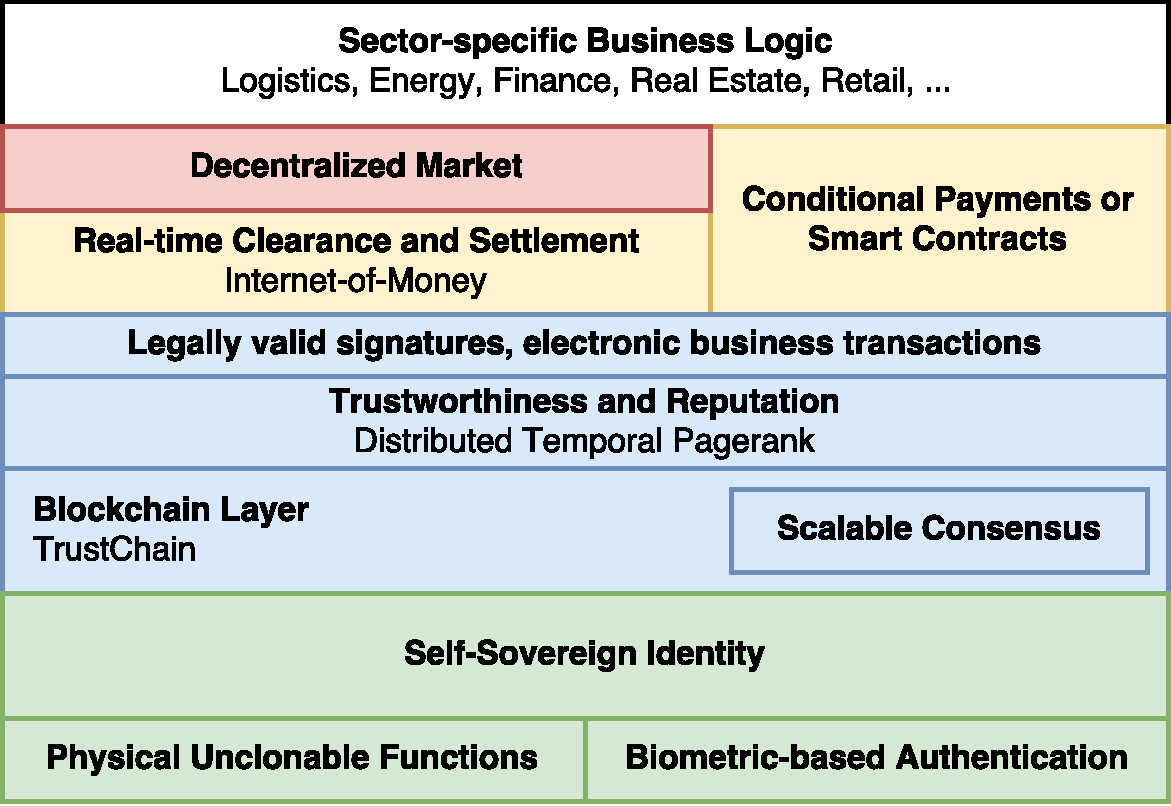
\includegraphics[width=.7\linewidth]{introduction/assets/tech_stack}
%	\caption{An overview of the research conducted at the Delft Blockchain Lab.}
%	\label{fig:dbl_tech_stack}
%\end{figure}

%\section{About the Delft Blockchain Lab}
%The Delft Blockchain lab is Delft's initiative for research, education and training in blockchain technology and trust on the Internet.
%Figure~\ref{fig:dbl_tech_stack} outlines the research directions of the Delft Blockchain Lab, ranging from low-level primitives like biometric-based authentication to sector-specific business logic.
%At the lowest layers (depicted in green), we build, deploy and evaluate new solutions for managing ones identity in the physical world and on the Internet.
%These solutions include biometric-based authentication and physical unclonable functions, a method to securely store a private key.
%A part of our ongoing research includes a self-sovereign identity solution that is currently being tested and deployed in the Netherlands.

%Our research effort around distributed ledger technology includes scalable consensus algorithms and Sybil-resistant reputation mechanisms.
%The TrustChain distributed ledger is presented in Chapter X.
%The other components of this thesis are mostly focussed on the research directions that are coloured yellow and red in Figure~\ref{fig:dbl_tech_stack}.
%For a detailed outline of our research efforts, we refer the reader to our published vision paper.

%\newpage

%\bibliographystyle{unsrt}
%\bibliography{introduction}